\documentclass[12pt,letterpaper]{report}
\usepackage[pdftex]{graphicx}
\usepackage[top=1in,bottom=1in,left=1in,right=1in]{geometry}
%\usepackage{fancyhdr}

%\setlength{\headheight}{15pt}
%\pagestyle{fancy}

\newcommand{\HRule}{\rule{\linewidth}{0.5mm}}

\begin{document}
 \flushleft
 \section*{CarbonTracker:}
  \subsection*{What it does:}
   \paragraph{}
	 CarbonTracker produces model predictions of atmospheric carbon dioxide ($CO_2$)  mole fractions, to be compared with the observed atmospheric $CO_2$ mole fractions. The difference between them is attributed to differences in the sources and sinks used to make the prediction (the so-called 'first-guess') and the sources and sinks affecting the true atmospheric $CO_2$. Using numerical techniques, these differences are used to solve for a set of sources and sinks that most closely matches the observed $CO_2$ in the atmosphere. CarbonTracker has a representation of atmospheric transport based on weather forecasts, and modules representing air-sea exchange of $CO_2$, photosynthesis and respiration by the terrestrial biosphere, and release of $CO_2$ to the atmosphere by fires and combustion of fossil fuels.
  \begin{center}
  \begin{minipage}{0.55\textwidth}
  \begin{flushleft}
  \ignorespaces
  {\large \textbf{Overview of process:}}
   \begin{enumerate}
	\item The Carbon Tracker initializes first
	with an estimation of the $CO_2$ distribution
	while	taking into account atmosphere sinks
	and sources.
	\item Then it is put in a model which
	simulates the air paths over the earth.
	\item The model is displayed.
	\item The estimated values of $CO_2$ are
	compared to the actual measurements of $CO_2$.
	\item The model is then corrected to show
	a better representation of the $CO_2$ distribution.
	\end{enumerate}
  \end{flushleft}
  \end{minipage}
  \begin{minipage}{7cm}
  \begin{flushright}
   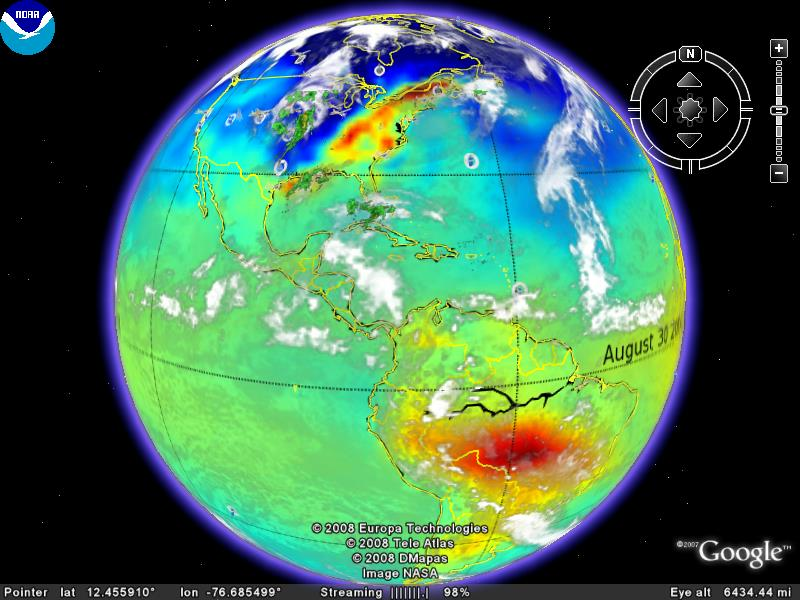
\includegraphics[width=7cm]{example}
	\begin{center}
	\tiny{Image taken using a CarbonTracker file made for Google earth}
	\end{center}
  \end{flushright}
  \end{minipage}
  \end{center}
 \section*{How to use or implement CarbonTracker:}
  \paragraph{}
   There are apparently seven modules/components that CarbonTracker utilizes in making its estimation for the model display.  The modules are Ocean, Fire, Biosphere, and Fossil Fuel and the other components are the Observations taken by NOAA ESRL and partner laboratories, the TM5 nested transport, and the Ensemble Data Assimilation.
	\subsection*{Ensemble Data Assimilation}
	 \begin{itemize}
	 \item The Ensemble Data Assimilation seems to be the heart of the work in CarbonTracker, it connects the information collected from each of the modules and the observations, and it updates the display periodically based upon changes in the data it takes in.
	 \item The equation used by this process to make sense of the fluxes in $CO_2$:\newline
	 F(x, y, t) = $\lambda \cdot F_{bio}$(x, y, t) + $\lambda \cdot F_{oce}$(x, y, t) + $F_{ff}$(x, y, t) + $F_{fire}$(x, y, t)
	 \item $lambda$ represents a set of linear scaling factors applied to the fluxes, which is estimated in the assimilation.  After the scaling factors are estimated they are then applied to the biosphere and ocean modules to determine the fluxes in output by CarbonTracker.
	 \item The scaling factors are estimated each week and assumed constant.
	  \begin{itemize}
	  \item[-] Each scaling factor is associated with a particular region, and the current distribution of regions is fixed.  
     \item[-] The ocean is divided into 30 basin regions, and the biosphere is divided according to the type of ecosystem and the geographical location.  
     \item[-] Since this project is intended to be used with a TransCom application, the number of separate locations is set to 11, and the number of ecosystems in each location is set to 19.  
     \item[-] CarbonTracker intentionally does not set scaling factors for the fossil fuel and fire modules.
	  \end{itemize}
	 \end{itemize}
	\subsection*{Observations}
	 \begin{itemize}
	 \item The observation data comes from air samples taken at the ground level from the NOAA ESRL Cooperative Air Sampling Network for each year studied.  The makeup of the network varies per week depending on successful sampling and analysis, and each site’s sampling frequency.
	 \item Data also comes from in situ quasi-continuous $CO_2$ time series from seven towers
	  \begin{description}
	  \item[-] The 396m level of the WLEF tower in Wisconsin
	  \item[-] The 107m level of the AMT tower in Argyle, Maine
	  \item[-] The 251m level of the KWKT tower in Texas
	  \item[-] The 40m level of the tower in Fraserdale, Canada operated by Environment Canada (EC)
	  \item[-] The 23m level of the tower at Candle Lake (formerly Old Black Spruce), Canada operated by EC
	  \item[-] The 9m level of the tower at Storm Peak Laboratory operated by National Center for Atmospheric Research (NCAR)
	  \item[-] The 5m level of the tower at Niwot Ridge operated by NCAR.
	  \item[-] There are other in situ quasi-continuous $CO_2$ time series that come from NOAA ESRL observatories at Barrow, Mauna Loa, Samoa, and South Pole, and the EC programs at Alert, Canada and Sable Island, Canada.
	  \end{description}
	 \item At the quasi-continuous sampling sites, one daytime average mole faction for each day is constructed from the time series.
	 \item During the assimilation a selection criterion to exclude non-Marine Boundary Layer observations from which are poorly forecasted in the framework.  A model-data mismatch is used in this process, which is the random error ascribed to each observation to account for measurement errors as well as modeling errors.
	 \end{itemize}
	\subsection*{Ocean Module}
	 \begin{itemize}
	 \item The oceans or the largest long-term sink for carbon and hold a massive capacity to store and redistribute $CO_2$ within a system.
	 \item It is estimated that 48\% of the $CO_2$ from fossil fuels has been absorbed by the ocean.
	 \item Oceanic uptake of $CO_2$ in CarbonTracker is computed using air-sea differences in partial pressure of $CO_2$ inferred from ocean inversions, combined with a gas transfer velocity computed from wind speeds in the atmospheric transport model.
	 \end{itemize}
	\subsection*{Biosphere}
	 \begin{itemize}
	 \item The biospheric component of the carbon cycle consists of all the carbon stored in 'biomass' around us. This includes trees, shrubs, grasses, carbon within soils, dead wood, and leaf litter.
	 \item This model calculates global carbon fluxes using input from weather models to drive biophysical processes, as well as satellite observed Normalized Difference Vegetation Index (NDVI) to track plant phenology.
	 \end{itemize}
	\subsection*{Fire Module}
	 \begin{itemize}
	 \item This important component of the carbon cycle is monitored mostly from space, while sophisticated 'biomass burning' models are used to estimate the amount of $CO_2$ emitted by each fire. Such estimates are then used in CarbonTracker to prescribe the emissions, without further refinement by measurements.
	 \item The fire module currently used in CarbonTracker is based on the Global Emissions Fire Database version 2 (GFEDv2), which is derived from the CASA biogeochemical model.  The dataset consists of $1\times1$ degree gridded monthly burned area, fuel loads, combustion completeness, and fire emissions (Carbon, $CO_2$, CO, $CH_4$, NMHC, $H_2$, $NO_x$, $N_2$O, PM2.5, Total Particulate Matter, Total Carbon, Organic Carbon, Black Carbon) for the time period spanning January 1997 - December 2006, of which only $CO_2$ is currently used.
	 \end{itemize}
	\subsection*{Fossil Fuel}
	 \begin{itemize}
	 \item Over the last two centuries, following the industrial and technical revolutions and the world population increase, fossil fuel combustion has become the largest anthropogenic source of $CO_2$.
	 \item Annual global total fossil fuel $CO_2$ emissions are from the Carbon Dioxide Information and Analysis Center (CDIAC) [Marland et al. 2006] which extend through 2004.
	 \item The uncertainty attached to the total source is of the order of 15\%. This source is not optimized in the current CarbonTracker as it is believed the current network cannot constrain this source separately from the others. Although the contribution of $CO_2$ from fossil fuel burning to the observed $CO_2$ mole fraction is considered known, extra model error is included in the system to represent the random errors in fossil fuels.
	 \end{itemize}
	\subsection*{TM5 Nested Transport}
	 \begin{itemize}
	 \item This is a community-supported model whose development is shared among many scientific groups with different areas of expertise.
	 \item TM5 is a global model with two-way nested grids; regions for which high-resolution simulations are desired can be nested in a coarser grid spanning the global domain. The advantage is that transport simulations can be performed with a regional focus without the need for boundary conditions from other models.
	 \item To simulate the winds and the weather, CarbonTracker uses sophisticated numerical models that are driven by the daily weather forecasts from the specialized meteorological centers of the world.  The winds which drive TM5 come from the European Center for Medium range Weather Forecast (ECMWF) operational forecast model.
	 \end{itemize}

 \begin{thebibliography}{1}
 \bibitem{pa} CarbonTracker 2007B, http://carbontracker.noaa.gov
 \end{thebibliography}
\end{document}

